\author{Sumedh Joshi}
\title{Spectral Multi-Domain Penalty Method Quick Start Guide}
\documentclass[onside]{article}
\usepackage{graphicx}
\usepackage{epstopdf}
\usepackage{fullpage}
\usepackage{microtype}

\begin{document}
\maketitle

This guide accompanies the Spectral Multi-Domain Penalty Method (SMPM) code.  It provides step-by-step instructions to create, run, and visualize an SMPM code run.

\section{Dependencies}

The SMPM code requires:
\begin{enumerate}
	\item gfortran or Intel's ifort fortran compiler
	\item BLAS and LAPACK
	\item HDF5 and its Fortran interface
	\item MPI
\end{enumerate}

To install these on Ubuntu 14.04 LTS execute the following command: 

	 \begin{verbatim} $ sudo apt-get install gfortran libblas3gf liblapack3gf\
	  hdf5-tools h5utils mpich2 \end{verbatim}

All of these packages are available on other Linux systems, but may have slightly different names; please consult your package manager to obtain them.

\section{Compilation}
\label{compile}

\subsection{Compiling with gfortran}

To compile with gfortran with the default compiler flags, type:

\begin{verbatim}
	$ make DEBUG=yes OPTIMIZE=yes FC90=gfortran FC90_WRAPPER=mpif90
\end{verbatim}

This compiles the code with optimizations and debugging flags turned on, and uses the default installation of LAPACK/BLAS in your /usr/lib directory.  Usually the LAPACK/BLAS installed there is slow, and if you have the freely available AMD's Core Math Library (ACML) you should use it.  

If your ACML is installed in the ACML\_ROOT directory, then compile with the following options to use it:
\begin{verbatim}
	$ make DEBUG=yes OPTIMIZE=yes FC90=gfortran FC90_WRAPPER=mpif90 \
	ACML_ROOT=/path/to/acml BLAS=ACML
\end{verbatim}

If no ACML\_ROOT or BLAS variable is issued at compile time, then the code assumes you wanted it to compile with the default LAPACK/BLAS installation.  

\subsection{Compiling with ifort}

If the Intel Fortran compiler is installed, then it is not necessary to provide specific directions to BLAS/LAPACK, as the Makefile will link against the Intel Math Kernel Library instead.  Compile with ifort with the following default flags:

\begin{verbatim}
	$ make DEBUG=yes OPTIMIZE=yes FC90=ifort FC90_WRAPPER=mpif90 
\end{verbatim}

\section{Operating the code}

\subsection{Input Files}

The SMPM code takes two input files which serve the following purpose:
\begin{enumerate}
	\item \textbf{Input File}: a text file that contains execution options, physical constants, output file names, etc.  This is an ASCII file that is case-insensitive and can be commented with \# as the comment character.
	\item \textbf{Initial Conditions File}: a binary HDF5 file that contains the grid and the initial conditions ($u_x, u_z, \rho, \bar{\rho}$ at time $t = t_0$ the start of the simulation).
\end{enumerate}

There are MATLAB file readers and writers for both the input and the init files in the /smpm\_matlab\_utilities directory.

\subsection{Output Files}

The code generates two output files:
\begin{enumerate}
	\item \textbf{Field File}: the field file is a binary HDF5 file in the VTK data format.  It contains the two velocities and density at each time-step.
	\item \textbf{XDMF File}: this is a text file that is generated so that VTK visualization tools such as Paraview, Visit, etc. can read the field file.
\end{enumerate}

There is MATLAB file reader and writer for the field file format, and there is a Python script that will automatically build the XDMF file from the field file.  The SMPM code will also automatically generate the xdmf file at the conclusion of a simulation. 

	\subsection{Meshing}
	
	Generation of meshes is done in one of several MATLAB scripts contained in the /smpm\_matlab\_utilities subfolder.  These are described briefly in Table \ref{meshing}, but you can always type ``$\gg$ help [meshing routine name]'' into the MATLAB command line to get detailed execution instructions.
	
\begin{table}[h]
\centering
\caption{A description of the four meshing routines provided, arranged from least (top) to most (bottom) complex.}
\label{meshing}
\begin{tabular}{lllll}
{\bf Name}                   & {\bf Description}                                                             &  &  &  \\
smpm\_build\_cartesian\_mesh & Construct a rectangular domain with uniformly-spaced elements.                      &  &  &  \\
smpm\_build\_kron\_mesh      & Construct a rectangular domain with unevenly-spaced but rectangular elements.       &  &  &  \\
smpm\_build\_bathy\_mesh     & Construct a domain by specifying a ocean bottom bathymetry.                         &  &  &  \\
smpm\_build\_layered\_mesh   & Construct a domain by specifying all of the horizontal interfaces between elements. &  &  & \end{tabular}
\end{table}
	
	We use the meshing routines to build vectors $x$ and $z$ that represent the grid.  For example, to build a uniformly spaced $8 \times 8$ element mesh with $4$ GLL points per direction on a rectangular domain of width 10 and height 5 units, we would type
	
	\begin{verbatim}
		>> [x z] = smpm_build_cartesian_mesh( 4, 8, 8, [0 10], [0 5] );
	\end{verbatim}
	
	Finally, note that the meshing routines provided are merely for convenience; you are free to define the grid vectors $x$ and $z$ however you wish, although the meshing routines will cover most meshes required.
	
	\subsection{Initial Conditions}
	
	Once you have meshed and created $x$ and $z$ you can create the initial values for $u_x, u_z, \rho, \bar{\rho}$ and write them into an initial conditions file by 
	\begin{verbatim}
		>> smpm_write_initfile( n, mx, mz, x, z, rho, ux, uz, rho_bar, init_file_name );
	\end{verbatim}
	
	Here, all of the variables are the same size and dimension as the $x$ and $z$ vectors we just assembled with one of the SMPM meshing routines.
	
	\subsection{Input File}
	
	The input file can also be generated in MATLAB as a struct, and written to disk with the MATLAB routine smpm\_write\_inputfile.  We'll look at an example of an input file later in the tutorials.
	
	\subsection{Execution}
	
	Having built an input file called ``case1.in", run the SMPM code by typing
	
	\begin{verbatim}
		$ mpiexec -np 4 ./smpm_incompressible_navier_stokes case1.in case1.out
	\end{verbatim}
	
	\subsection{Visualization}

   The SMPM code will generate two output files.  The first is an HDF5 file called ``field" file, and has the extension .h5.  This field file contains the grid, $u_x$, $u_z$, and $\rho$ for all the time timesteps.  It is the primary data storage file, and is called a \emph{field} file because it stores all of the field variables.  You can load the field file (and any subsets of time-steps) in MATLAB using the provided MATLAB function smpm\_read\_fieldfile that is located in the /smpm\_matlab\_utilities folder.  Read the help documentation of this function for more information.

   The second file generated is a plain-text XDMF file and has the extension .xmf.  This file contains meta-data about the field file that can be used to visualize the results in any visualization software that can read XDMF format data.  One good example is Paraview\footnote{I think tecplot can also read XDMF data but I am not sure}.  To load the .xmf file in Paraview, open Paraview and go to file $>$ open and open the .xmf file.  The SMPM code automatically generates the .xmf file at the end of the simulation.  If \emph{during} a simulation you want to create an .xmf file and view it in Paraview, use the provided smpm\_create\_xdmf.py function that is located in the main source directory as follows:
	\begin{verbatim}
		./smpm_create_xdmf.py [field file name].h5 > [xmf file name].xmf
	\end{verbatim}
   where you replace the field file name with the field file that is currently being written to.  Then open the .xmf file using Paraview.  Paraview has many visualization tutorials to help you build graphics with this data.


\section{Examples}

In the /examples folder are some example cases.  In each folder are two files: the first is a MATLAB file that sets up all the necessary inputs for the SMPM code; the second is a shell script that uses those input files and executes the SMPM code.  Obviously run the MATLAB file first to build the inputs, and then use the provided shell script to execute the SMPM code.

The MATLAB files are heavily commented and intended to be used as tutorials or templates for your own simulations.  At the end of each of these simulations, you can open the ``.xmf'' file that will be generated in ParaView to visualize the results, or you can open the ``.h5'' field file in MATLAB using the ``smpm\_read\_fieldfile'' function in the /smpm\_matlab\_utilities folder.

\subsection{examples/ex01\_lid\_driven\_cavity}

The lid-driven cavity is a benchmark unstratified fluid flow problem.  It is a simple problem that demonstrates how to set boundary conditions, initial conditions, and build a cartesian mesh.  Run the MATLAB script in the lid-driven cavity example folder to build all the input files.

At this point you may want to look at the input file ``lid\_driven\_cavity\_in'' we just generated.  Recall that it is just an ASCII text file
that can be commented with \# as the comment character, and is case-insensitive.  

While you can use the shell script in the examples/ex01\_lid\_driven\_cavity to run the SMPM code, this is a short enough test case that you can also just run it from the command line.  To execute the SMPM code with 4 MPI ranks (assuming you have compiled it c.f. Section \ref{compile}) type
\begin{verbatim}
$ mpiexec -np 4 ./smpm_incompressible_navier_stokes \
                               lid_driven_cavity_in \
                               lid_driven_cavity_out
\end{verbatim}
The input file will be read and a field file called lid\_driven\_cavity.h5 will be generated in this directory.  There are several ways to visualize the field file.  Perhaps the most straightforward for this run is to just read it into Matlab.

\subsubsection{Reading a field file in MATLAB}

Open up a MATLAB session and navigate to the directory in which you just executed the SMPM code.  Make sure you have added the /smpm\_matlab\_utilities folder to your path using the MATLAB function addpath.

To read the entirety of the field file, type
\begin{verbatim}
>> data = smpm_read_fieldfile( 'lid_driven_cavity.h5' )

data = 

     grid: [1x1 struct]
    field: [1x1 struct]
\end{verbatim}
As you can see, data is a MATLAB structure with two substructures.  The grid substructure contains, predictably, the grid functions, and the field substructure contains the field variables ($u_x,u_z,\rho$) at every time step, stored in a 3D array.

\begin{verbatim}
>> data.grid

ans = 

     x: [128x128 double]
     z: [128x128 double]
     n: 8
    mx: 16
    mz: 16
    
>> data.field

ans = 

     ux: [128x128x100 double]
     uz: [128x128x100 double]
    rho: [128x128x100 double]

\end{verbatim}

Let's visualize this data along with the grid.  First, to visualize the $x$ velocity field at the last time-step use MATLAB's contourf function (and add a color bar):
\begin{verbatim}
>> contourf(data.grid.x,data.grid.z,data.field.ux(:,:,end));
>> colorbar;
\end{verbatim}
To overlay the SMPM element grid onto this field use the SMPM mesh visualizer:
\begin{verbatim}
>> smpm_visualize_mesh( data.grid.n, data.grid.mx, data.grid.mz, data.grid.x, data.grid.z, gcf);	
\end{verbatim}
The resulting image should look something like Fig.~\ref{ldc}
\begin{figure}
	\begin{center}
	\label{ldc}
	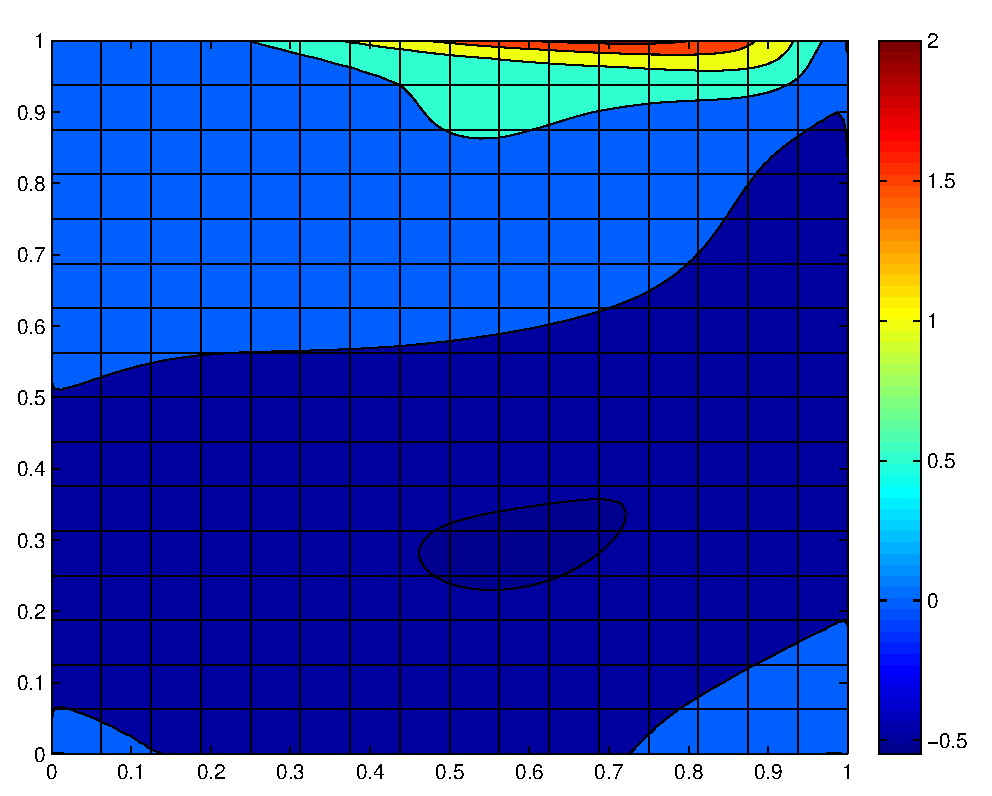
\includegraphics[width=0.5\textwidth]{quickstart_lid_driven_cavity_ux.eps}
	\end{center}
	\caption{The $u_x$ velocity resulting from the simulation of the lid driven cavity case up to time $t = 0.03$ seconds.}
\end{figure}

Note that if we just wanted to read the last time-step of this simulation, we could pass a second argument to the field file reader in MATLAB and read just the last time-step's worth of data by typing:
\begin{verbatim}
>> data = smpm_read_fieldfile( 'lid_driven_cavity.h5', -1 );
\end{verbatim}

You can similarly read in the first few time steps, the last few time steps, or a random scattering of time-steps as follows:
\begin{verbatim}
>> data = smpm_read_fieldfile( 'lid_driven_cavity.h5', [1:10] );
>> data = smpm_read_fieldfile( 'lid_driven_cavity.h5', [-1:-1:-10] );
>> data = smpm_read_fieldfile( 'lid_driven_cavity.h5', [1 25 -25 10 -1] );
\end{verbatim}

\subsection{/examples/ex02\_lock\_exchange}

The stratified lock exchange problem is an example incompressible flow that has non-constant density.  It has a non-uniform mesh that is finely sampled near the density jump.

Because this simulation can take some time, It is advisable to run the lock exchange problem with the Linux screen command as follows:

\begin{verbatim}
$ screen
$ ./run_ex02_lock_exchange.sh
\end{verbatim}
and then type CTRL-A followed by CTRL-D to detach the screen.  You can always follow the progress of the lock exchange simulation by
examining the ``lock\_exchange\_log'' file that will be generated in the current directory.  Running with the screen command allows you to
logout of your current session without terminating the execution of the SMPM code.  For simulation that will take a long time, this is
the preferred mode of execution.

After running this simulation, open the lock\_exchange\_out.xmf file in Paraview to see a visualization of the density and the two velocities.  Of course you can also open the field file, lock\_exchange\_out.h5, using smpm\_read\_fieldfile.m in MATLAB to visualize and post-process the lock exchange run.

\subsection{/examples/ex03\_shoaling\_internal\_wave}

This test case represents a physical simulation of a shoaling nonlinear internal wave.  The bathymetric data is taken from near the Dongsha island in the South China Sea, and the initial disturbance is taken from the solution of the Dubreil-Jacotin-Long (DJL) eigenvalue problem.  This tutorial shows how to take bathymetric data and use it to build a domain and mesh, take a simulation from the DJL solver and interpolate it onto this mesh, initialize the initial conditions and input files, and run such a shoaling simulation.  As such, this tutorial/example is a good jumping-off point for other deformed domain simulations of internal waves you might want to do.

Just like the lock-exchange problem, it is advisable to run the shoaling internal wave test case in a screen session (see previous example).  And, like all the SMPM simulations, you can visualize the output by opening the .h5 file in MATLAB using smpm\_read\_fieldfile or by opening the associated .xmf file in Paraview.


\end{document}
